% questions.tex —— 2024 年·新高考Ⅱ卷 · 题目内容片段（无答案）
% 由 tools/generate_projects.py 依来源总账自 2024/2024_数学真题_新高考Ⅱ_试题.md 生成，勿手改（改源 MD 后重跑）


\begin{gknotice}
\textbf{结构分水岭}：2024 年起题量由 22 题减为 19 题（多选 4→3、填空 4→3、解答 6→5），单题分值提高、压轴更难。本卷结构与 2025、2026 完全一致，\textbf{是最贴近 2027 高考的对标真题之一}。

\textbf{适用省份}：辽宁、重庆、海南、吉林、黑龙江、山西、云南、广西、甘肃、贵州、新疆

\textbf{来源说明}：试题原文取自 deekur/gaokaomath（commit \texttt{34c13a6}，CC BY 4.0）之「2024新高考2」PDF，逐题照图转录。
\end{gknotice}

\par\medskip

\gkpart{一、单选题}

\begin{gktip}
本题共 8 小题，每小题 5 分，共 40 分。在每小题给出的四个选项中，只有一项是符合题目要求的。
\end{gktip}

\begin{question}
\gkti{1}已知 $z=-1-\mathrm i$，则 $|z|=$\mbox{（　　）}

\begin{gkopts}(4)
\task A．$0$
\task B．$1$
\task C．$\sqrt2$
\task D．$2$
\end{gkopts}

\end{question}
\begin{question}
\gkti{2}已知命题 $p$：$\forall x\in\mathbf R$，$|x+1|>1$；命题 $q$：$\exists x>0$，$x^{3}=x$。则\mbox{（　　）}

\begin{gkopts}(2)
\task A．$p$ 和 $q$ 都是真命题
\task B．$\neg p$ 和 $q$ 都是真命题
\task C．$p$ 和 $\neg q$ 都是真命题
\task D．$\neg p$ 和 $\neg q$ 都是真命题
\end{gkopts}

\end{question}
\begin{question}
\gkti{3}已知向量 $\boldsymbol a$，$\boldsymbol b$ 满足 $|\boldsymbol a|=1$，$|\boldsymbol a+2\boldsymbol b|=2$，且 $(\boldsymbol b-2\boldsymbol a)\perp\boldsymbol b$，则 $|\boldsymbol b|=$\mbox{（　　）}

\begin{gkopts}(2)
\task A．$\dfrac12$
\task B．$\dfrac{\sqrt2}2$
\task C．$\dfrac{\sqrt3}2$
\task D．$1$
\end{gkopts}

\end{question}
\begin{question}
\gkti{4}某农业研究部门在面积相等的 $100$ 块稻田上种植一种新型水稻，得到各块稻田的亩产量（单位：kg）并整理得下表：

\begin{center}
\begin{tabular}{cccc}
\toprule
亩产量 & $[900,950)$ & $[950,1000)$ & $[1000,1050)$ \\
\midrule
频数 & $6$ & $12$ & $18$ \\
\bottomrule
\end{tabular}
\end{center}

\begin{center}
\begin{tabular}{cccc}
\toprule
亩产量 & $[1050,1100)$ & $[1100,1150)$ & $[1150,1200)$ \\
\midrule
频数 & $30$ & $24$ & $10$ \\
\bottomrule
\end{tabular}
\end{center}

  根据表中数据，下列结论中正确的是\mbox{（　　）}

\begin{gkopts}(1)
\task A．$100$ 块稻田亩产量的中位数小于 $1050$ kg
\task B．$100$ 块稻田中亩产量低于 $1100$ kg 的稻田所占比例超过 $80\%$
\task C．$100$ 块稻田亩产量的极差介于 $200$ kg 至 $300$ kg 之间
\task D．$100$ 块稻田亩产量的平均值介于 $900$ kg 至 $1000$ kg 之间
\end{gkopts}

\end{question}
\begin{question}
\gkti{5}已知曲线 $C:x^{2}+y^{2}=16\ (y>0)$，从 $C$ 上任意一点 $P$ 向 $x$ 轴作垂线段 $PP'$，$P'$ 为垂足，则线段 $PP'$ 的中点 $M$ 的轨迹方程为\mbox{（　　）}

\begin{gkopts}(2)
\task A．$\dfrac{x^{2}}{16}+\dfrac{y^{2}}4=1\ (y>0)$
\task B．$\dfrac{x^{2}}{16}+\dfrac{y^{2}}8=1\ (y>0)$
\task C．$\dfrac{y^{2}}{16}+\dfrac{x^{2}}4=1\ (y>0)$
\task D．$\dfrac{y^{2}}{16}+\dfrac{x^{2}}8=1\ (y>0)$
\end{gkopts}

\end{question}
\begin{question}
\gkti{6}设函数 $f(x)=a(x+1)^{2}-1$，$g(x)=\cos x+2ax$。当 $x\in(-1,1)$ 时，曲线 $y=f(x)$ 与 $y=g(x)$ 恰有一个交点。则 $a=$\mbox{（　　）}

\begin{gkopts}(4)
\task A．$-1$
\task B．$\dfrac12$
\task C．$1$
\task D．$2$
\end{gkopts}

\end{question}
\begin{question}
\gkti{7}已知正三棱台 $ABC\text{-}A_1B_1C_1$ 的体积为 $\dfrac{52}3$，$AB=6$，$A_1B_1=2$，则 $A_1A$ 与平面 $ABC$ 所成角的正切值为\mbox{（　　）}

\begin{gkopts}(4)
\task A．$\dfrac12$
\task B．$1$
\task C．$2$
\task D．$3$
\end{gkopts}

\end{question}
\begin{question}
\gkti{8}设函数 $f(x)=(x+a)\ln(x+b)$。若 $f(x)\ge0$，则 $a^{2}+b^{2}$ 的最小值为\mbox{（　　）}

\begin{gkopts}(4)
\task A．$\dfrac18$
\task B．$\dfrac14$
\task C．$\dfrac12$
\task D．$1$
\end{gkopts}

\par\medskip

\end{question}
\gkpart{二、多选题}

\begin{gktip}
本题共 3 小题，每小题 6 分，共 18 分。全部选对得 6 分，部分选对得部分分，有选错得 0 分。
\end{gktip}

\begin{question}
\gkti{9}对于函数 $f(x)=\sin2x$ 和 $g(x)=\sin\left(2x-\dfrac\pi4\right)$，下列说法中正确的有\mbox{（　　）}

\begin{gkopts}(2)
\task A．$f(x)$ 与 $g(x)$ 有相同的零点
\task B．$f(x)$ 与 $g(x)$ 有相同的最大值
\task C．$f(x)$ 与 $g(x)$ 有相同的最小正周期
\task D．$f(x)$ 与 $g(x)$ 的图象有相同的对称轴
\end{gkopts}

\end{question}
\begin{question}
\gkti{10}抛物线 $C:y^{2}=4x$ 的准线为 $l$，$P$ 为 $C$ 上动点。过 $P$ 作 $\odot A:x^{2}+(y-4)^{2}=1$ 的一条切线，$Q$ 为切点。过 $P$ 作 $l$ 的垂线，垂足为 $B$。则\mbox{（　　）}

\begin{gkopts}(1)
\task A．$l$ 与 $\odot A$ 相切
\task B．当 $P$，$A$，$B$ 三点共线时，$|PQ|=\sqrt{15}$
\task C．当 $|PB|=2$ 时，$PA\perp AB$
\task D．满足 $|PA|=|PB|$ 的点 $P$ 有且仅有 $2$ 个
\end{gkopts}

\end{question}
\begin{question}
\gkti{11}设函数 $f(x)=2x^{3}-3ax^{2}+1$，则\mbox{（　　）}

\begin{gkopts}(1)
\task A．当 $a>1$ 时，$f(x)$ 有三个零点
\task B．当 $a<0$ 时，$x=0$ 是 $f(x)$ 的极大值点
\task C．存在 $a$，$b$，使得 $x=b$ 为曲线 $y=f(x)$ 的对称轴
\task D．存在 $a$，使得点 $\left(1,f(1)\right)$ 为曲线 $y=f(x)$ 的对称中心
\end{gkopts}

\par\medskip

\end{question}
\gkpart{三、填空题}

\begin{gktip}
本题共 3 小题，每小题 5 分，共 15 分。
\end{gktip}

\begin{question}
\gkti{12}记 $S_n$ 为等差数列 $\left\{a_n\right\}$ 的前 $n$ 项和。若 $a_3+a_4=7$，$3a_2+a_5=5$，则 $S_{10}=$ \gkblank{}．

\end{question}
\begin{question}
\gkti{13}已知 $\alpha$ 为第一象限角，$\beta$ 为第三象限角，$\tan\alpha+\tan\beta=4$，$\tan\alpha\tan\beta=\sqrt2+1$，则 $\sin(\alpha+\beta)=$ \gkblank{}．

\end{question}
\begin{question}
\gkti{14}在如图的 $4\times4$ 的方格表中选 $4$ 个方格，要求每行和每列均恰有一个方格被选中，则共有 \gkblank{} 种选法。在所有符合上述要求的选法中，选中方格中的 $4$ 个数之和的最大值是 \gkblank{}．

\begin{center}
\begin{tabular}{cccc}
\toprule
 &  &  &  \\
\midrule
$11$ & $21$ & $31$ & $40$ \\
$12$ & $22$ & $33$ & $42$ \\
$13$ & $22$ & $33$ & $43$ \\
$15$ & $24$ & $34$ & $44$ \\
\bottomrule
\end{tabular}
\end{center}

\par\medskip

\end{question}
\gkpart{四、解答题}

\begin{gktip}
本题共 5 小题，共 77 分。解答应写出文字说明、证明过程或演算步骤。
\end{gktip}

\begin{question}
\gkti{15}\textbf{（13 分）} 记 $\triangle ABC$ 的内角 $A$，$B$，$C$ 的对边分别为 $a$，$b$，$c$，已知 $\sin A+\sqrt3\cos A=2$。

  (1) 求 $A$；

  (2) 若 $a=2$，$\sqrt2\,b\sin C=c\sin2B$，求 $\triangle ABC$ 的周长。

\end{question}
\begin{question}
\gkti{16}\textbf{（15 分）} 已知函数 $f(x)=\mathrm e^{x}-ax-a^{3}$。

  (1) 当 $a=1$ 时，求曲线 $y=f(x)$ 在点 $\left(1,f(1)\right)$ 处的切线方程；

  (2) 若 $f(x)$ 有极小值，且极小值小于 $0$，求 $a$ 的取值范围。

\Needspace{0.4\textheight}
\end{question}
\begin{question}
\gkti{17}\textbf{（15 分）} 如图，平面四边形 $ABCD$ 中，$AB=8$，$CD=3$，$AD=5\sqrt3$，$\angle ADC=90^{\circ}$，$\angle BAD=30^{\circ}$，点 $E$，$F$ 满足 $\overrightarrow{AE}=\dfrac25\overrightarrow{AD}$，$\overrightarrow{AF}=\dfrac12\overrightarrow{AB}$，将 $\triangle AEF$ 沿 $EF$ 翻折至 $\triangle PEF$，使得 $PC=4\sqrt3$。
\nopagebreak[4]
\begin{center}% 2024 新高考Ⅱ卷 17：矩形沿 EF 翻折后的立体（P 为翻起的 A 点新位置）
% 绘制依据：转录 agent 自源 PDF 逐边核对的构型——立体坐标 E(0,0,0)、D(3√3,0,0)、
% F(0,2,0)、B(2√3,4,0)、C(3√3,3,0)、P(0,0,2√3)，折前 A(-2√3,0,0) 保留示折痕来源；
% 实线 A-E、A-F、F-B、B-C、C-D、P-F、P-B、P-C、P-D，虚线 E-D、E-F、P-E。
% 画布投影：(x,y,z) -> x·(1,0.13) + y·(-0.275,-0.525) + z·(0,0.9)
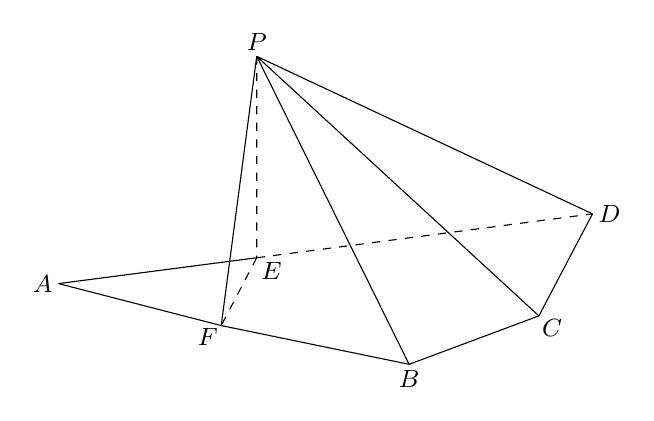
\begin{tikzpicture}[scale=0.82, font=\small]
  \coordinate (A) at (-3.07,-0.40);
  \coordinate (E) at (0,0);
  \coordinate (D) at (5.20,0.68);
  \coordinate (F) at (-0.55,-1.05);
  \coordinate (B) at (2.36,-1.65);
  \coordinate (C) at (4.37,-0.90);
  \coordinate (P) at (0,3.12);
  \draw (A) -- (E)  (A) -- (F);
  \draw (F) -- (B) -- (C) -- (D);
  \draw (P) -- (F)  (P) -- (B)  (P) -- (C)  (P) -- (D);
  \draw[dashed] (E) -- (D)  (E) -- (F)  (P) -- (E);
  \node[left, inner sep=2pt] at (A) {$A$};
  \node[below right, inner sep=1.5pt] at (E) {$E$};
  \node[right, inner sep=2pt] at (D) {$D$};
  \node[below left, inner sep=1pt] at (F) {$F$};
  \node[below, inner sep=2pt] at (B) {$B$};
  \node[below right, inner sep=1pt] at (C) {$C$};
  \node[above, inner sep=2pt] at (P) {$P$};
\end{tikzpicture}\end{center}
\nopagebreak[4]
  (1) 证明：$EF\perp PD$；

  (2) 求面 $PCD$ 与面 $PBF$ 所成的二面角的正弦值。

\end{question}
\begin{question}
\gkti{18}\textbf{（17 分）} 某投篮比赛分为两个阶段，每个参赛队由两名队员组成。比赛具体规则如下：第一阶段由参赛队中一名队员投篮 $3$ 次，若 $3$ 次都未投中，则该队被淘汰，比赛成绩为 $0$ 分；若至少投中 $1$ 次，则该队进入第二阶段。第二阶段由该队的另一名队员投篮 $3$ 次，每次投篮投中得 $5$ 分，未投中得 $0$ 分。该队的比赛成绩为第二阶段的得分总和。某参赛队由甲、乙两名队员组成，设甲每次投中的概率为 $p$，乙每次投中的概率为 $q$，各次投中与否相互独立。

  (1) 若 $p=0.4$，$q=0.5$，甲参加第一阶段比赛，求甲、乙所在队的比赛成绩不少于 $5$ 分的概率；

  (2) 假设 $0<p<q$。

  　① 为使得甲、乙所在队的比赛成绩为 $15$ 分的概率最大，应该由谁参加第一阶段比赛？

  　② 为使得甲、乙所在队的比赛成绩的数学期望最大，应该由谁参加第一阶段比赛？

\end{question}
\begin{question}
\gkti{19}\textbf{（17 分）} 已知双曲线 $C:x^{2}-y^{2}=m\ (m>0)$，点 $P_1(5,4)$ 在 $C$ 上，$k$ 为常数，$0<k<1$。按照如下方式依次构造点 $P_n\ (n=2,3,\cdots)$：过点 $P_{n-1}$ 作斜率为 $k$ 的直线与 $C$ 的左支交于点 $Q_{n-1}$，令 $P_n$ 为 $Q_{n-1}$ 关于 $y$ 轴的对称点。记 $P_n$ 的坐标为 $\left(x_n,y_n\right)$。

  (1) 若 $k=\dfrac12$，求 $x_2$，$y_2$；

  (2) 证明：数列 $\left\{x_n-y_n\right\}$ 是公比为 $\dfrac{1+k}{1-k}$ 的等比数列；

  (3) 设 $S_n$ 为 $\triangle P_nP_{n+1}P_{n+2}$ 的面积。证明：对于任意正整数 $n$，$S_n=S_{n+1}$。

\par\medskip

\begin{gktip}
\textbf{试题来源}：deekur/gaokaomath（commit \texttt{34c13a6}，CC BY 4.0）之「2024新高考2」PDF。
\end{gktip}

\end{question}